\section{Introduction}

Floating-point arithmetic is widely used
  in scientific, engineering, and graphical applications
  to approximate arithmetic on real numbers;
  typically, it is the
  only practical option available.%
\footnote{
  While alternatives exist,
    e.g., arbitrary-precision arithmetic,
    exact rational arithmetic,
    and constructive real arithmetic,
    they are orders of magnitude slower
    than hardware floating-point,
    and are thus inappropriate for many applications.
}
However, floating-point arithmetic must be used with care,
  as rounding errors can cause floating-point arithmetic
  and real-number arithmetic to give dramatically different results.
For example,
  naïve implementations of
  well-known mathematical equations like the quadratic formula
  can exhibit unacceptably-high rounding error (\Cref{fig:quadp-error}).
Rounding error can also ruin results
  for even extremely simple expressions.
\Cref{fig:cancellation} shows that,
  for large floating-point values of \texttt{x},
  the expression \texttt{x + 1 - x} can evaluate to 0
  instead of the mathematically correct 1!
Floating-point rounding error has caused
  unreproducible scientific research,
  distorted stock market indices,
  and wartime casualties~\cite{num-replication,distort-stock,patriot,euro-rounding,wall-street-distort-stock,num-issues-in-stat,round-elections}.

As a specific example, 
  a major bug in the implementation of \textit{asinh}/\textit{acosh} 
  in the Rust standard math library went unnoticed for seven years.
An automated test suite caught the bug in 2022 \cite{herbie-rust}.

% Physicists, mathematicians, aeronautics engineers,
%   machinists, AI engineers, and 3D artists
%   all run into floating-point error
%   at some point in their career.
In order to diagnose and repair this kind of error,
  \textit{numerical analysis experts} have developed
  techniques and tools for analyzing and rewriting 
  floating-point expressions over the last decade.
These tools support and facilitate automated
  test generation ~\cite{s3fp},
  error analysis ~\cite{gappa,vmcai11-fluctuat,daisy,satire,fm15-fptaylor},
  and repair ~\cite{salsa,herbie}.
For example,
  the open-source, state-of-the-art Herbie tool~\cite{herbie} takes as input a floating-point expression
  and uses algebraic and analytic identities to rewrite the expression
  via a complex search process.
Despite wide adoption of tools like Herbie in
  industrial and national labs,
  users still find results are too complicated and that
  tools overlook seemingly obvious rewritings.
  
  % ,
  % reporting that it does not work for their use case,
  % that its results are too complicated to trust,
  % or that it misses rewritings they see as obvious.
% Reducing floating-point rounding error is difficult, 
%   but not impossible for
%   \textit{numerical analysis experts}, who % \textit{can} deal with rounding error,
%   use algebraic and analytic identities
%   to rewrite floating-point expressions
%   into equivalent expressions with lower rounding error.
% However, even for experts,
%   diagnosing rounding error and coming up with solutions
%   is a difficult task 
%   that can take hours of work for a single expression.
% While the average programmer may correctly suppose 
%   that their application is not worth a formal numerical analysis
%   and often be right,
%   they may also incorrectly suppose the same thing 
%   with catastrophic results.
% Experienced numerical programmers 
%   confront this problem frequently and
%   regard floating-point arithmetic with justified suspicion.
  % and even these programmers are often taken by surprise.
  % but a major concern with floating point is that 
  % rounding errors can not be "caught" by a programmer,
  % so it is easy to underestimate their prevalence and impact in less
  % studied domains. 
  % Any program where numbers may become very 
  % large or small during evaluation is at risk, 
  % but since calculations occur without throwing errors,
  % it's easy to underestimate the effects,
  % and this becomes especially obvious in high-performance systems.


% Floating-point error is often \textit{silent}:
%   the computation will produce a result,
%   without signalling anything has gone awry,
%   but the result will be unacceptably wrong.
% Even when an error is signaled,
%   such as when a computation returns NaN
%   or attempts an invalid computation
%   like the square root of a negative number,
%   users may not have any alternative to floating-point arithmetic.
% The expression being computed may come from a paper or online reference
%   that does not provide an analysis of rounding error,
%   and few programmers are equipped to perform such analyses manually.

% For example, 
%   a major bug in the implementation of \textit{asinh}/\textit{acosh} 
%   in the Rust standard math library went unnoticed for 7 years
%   before finally being caught in 2022 
%   by an automated test suite \cite{herbie-rust}.

\lstset{escapeinside={<@}{@>}}

\begin{figure}
  \centering
  \begin{subfigure}[b]{0.4\textwidth} 
    \begin{lstlisting}[language=Python,commentstyle=\color{blue}] 
      # FP arithmetic seems ok
      >>> x = 1e15
      >>> x + 1 - x
      1.0

      # ... until it doesn't!
      >>> x = 1e16
      >>> x + 1 - x
      <@\textcolor{red}{\large 0.0}@>
    \end{lstlisting}
% 
    \caption{
      Example of ``catastrophic cancellation'' in Python. \\[8pt]
    }
    \label{fig:cancellation}
  \end{subfigure}
  \hfill
  \begin{subfigure}[b]{0.45\textwidth}

    %\shadowimage[width=0.9\columnwidth]{figures/quadp-error.png}
    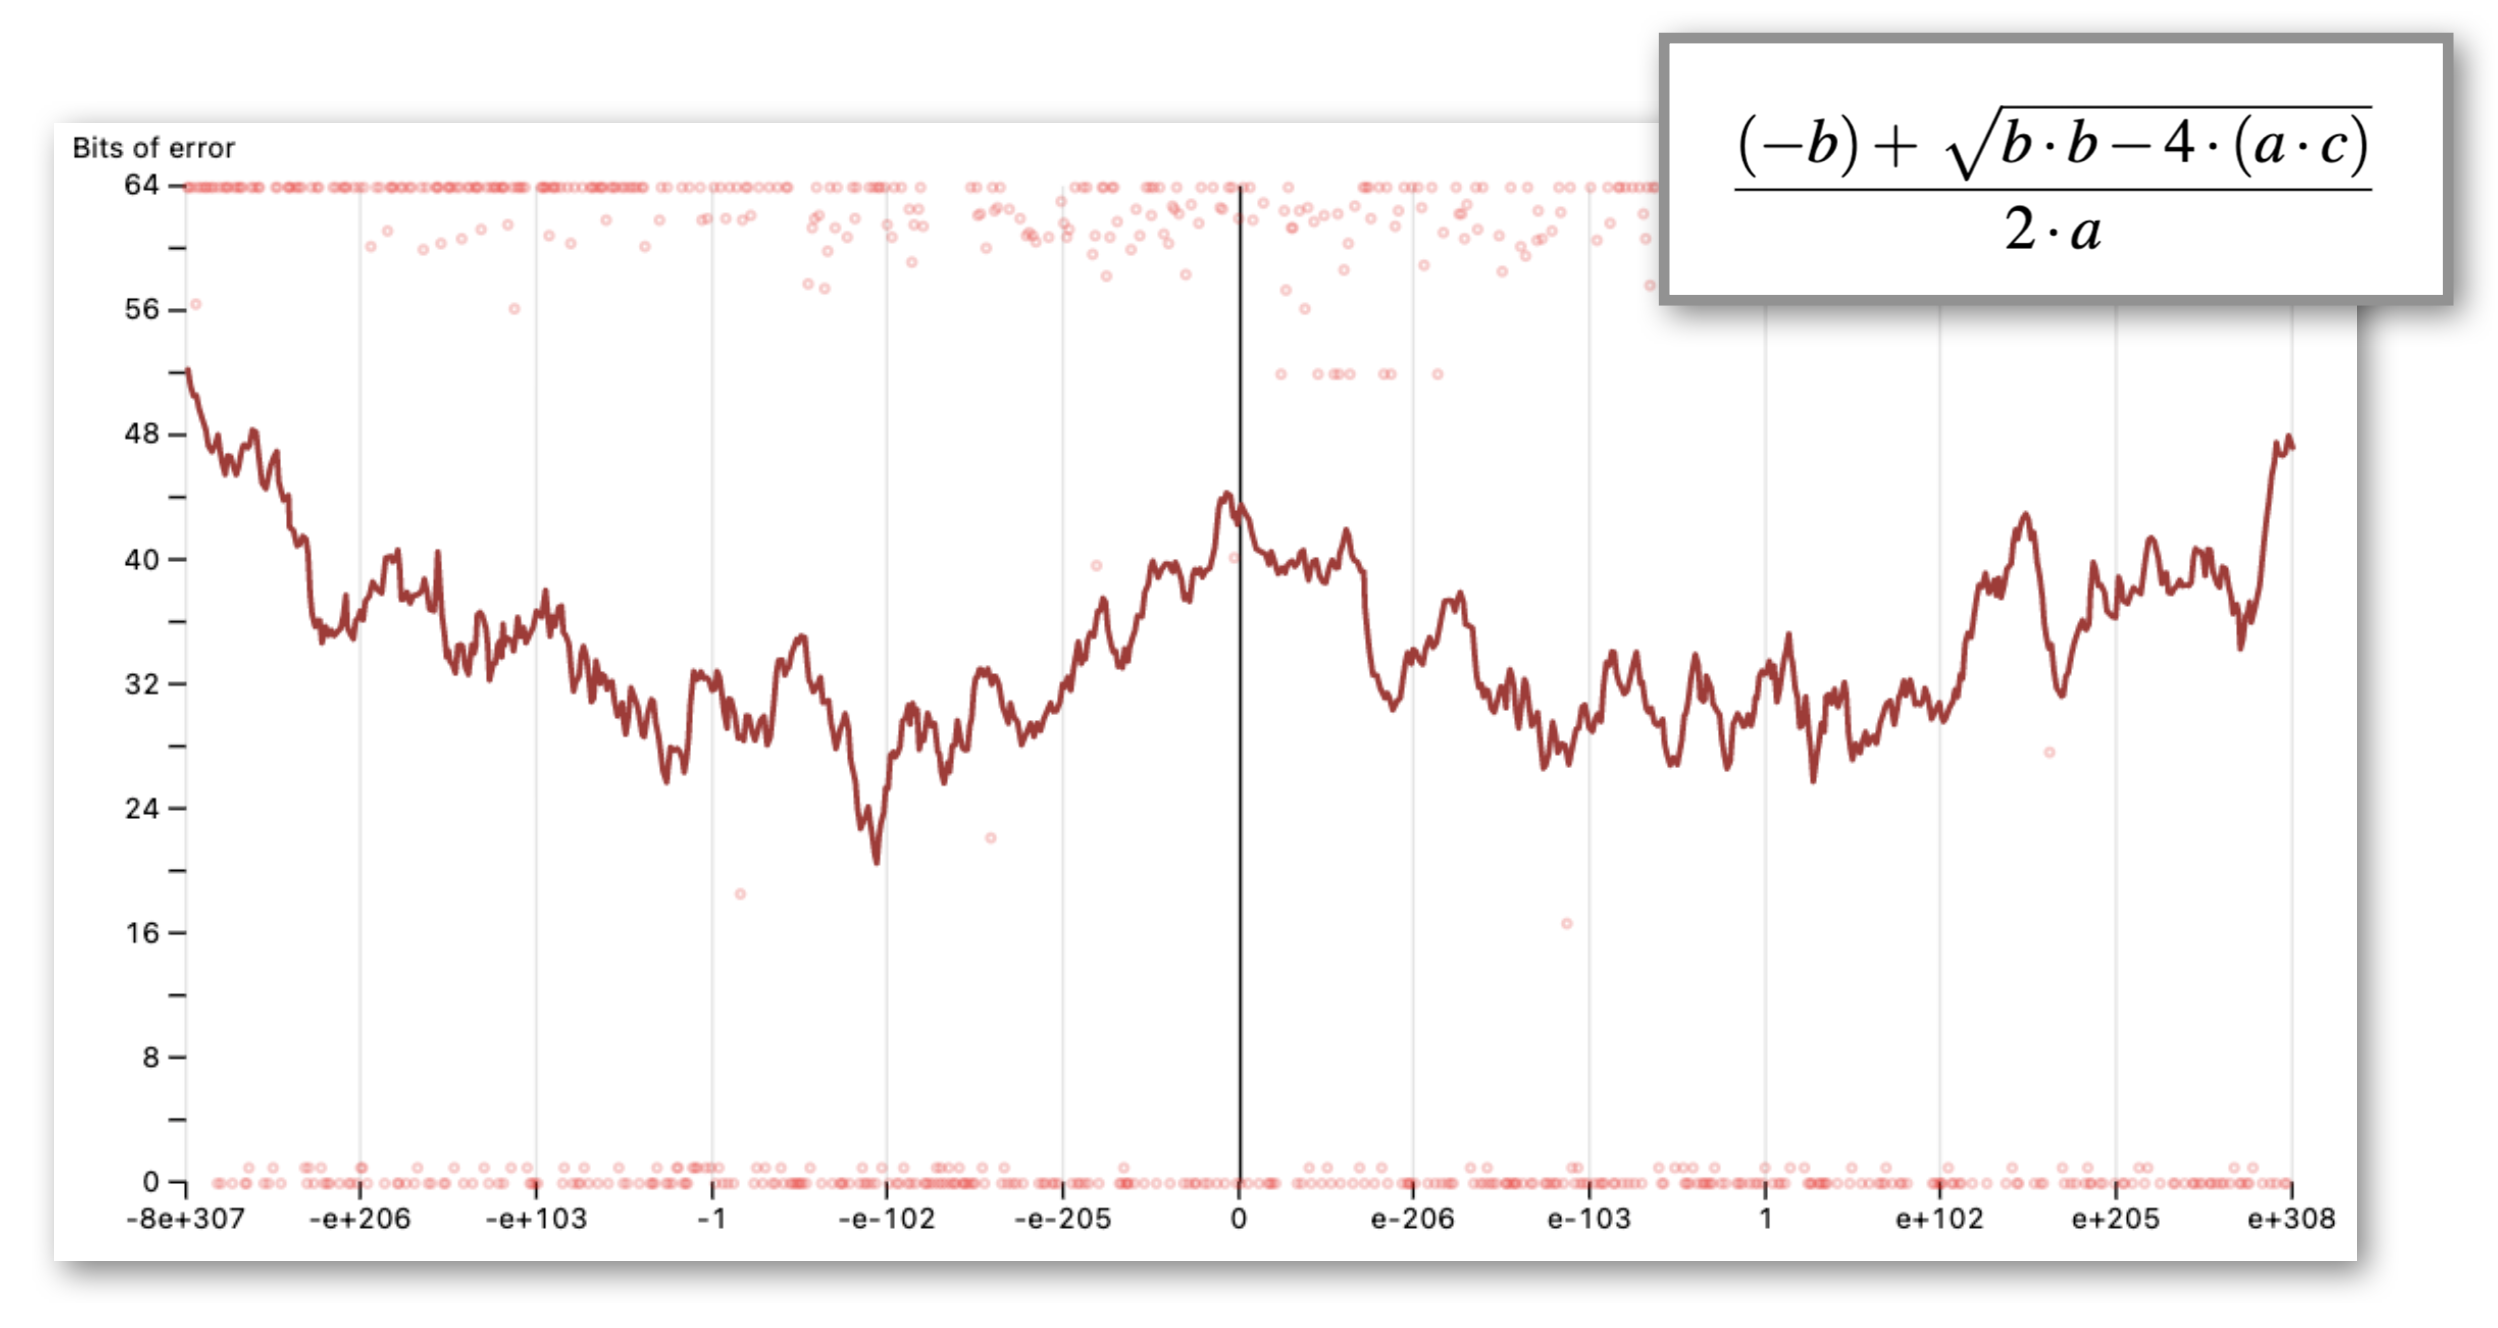
\includegraphics[width=\textwidth]{figures/quadp-error-with-eqn.png}
    \caption{
      Average ``bits'' 
        ($\log_2(\mathit{ulps})$)  
        of floating-point error
        with respect to $b$
        when evaluating the quadratic equation over
        randomly-sampled inputs.
      For many applications the error is unacceptable,
        but few programmers are equipped
        to address such numerical issues.
    }
    \label{fig:quadp-error}
  \end{subfigure}
  \caption{
    Floating-point error is pernicious;
      even familiar, simple expressions
      can yield meaningless results.
  }
\end{figure}

Fully understanding and fixing the bug in Rust required
  rewriting the naive definition $log(x + sqrt(x^2 + 1))$ as
  $log1p(x + x/(hypot(1, x) + x))$.
To arrive at the solution,
  numerical analysts needed to 
  repurpose internal operations of existing tools
  and apply their own expert knowledge.
\textbf{This example illustrates how experts must work with a constellation 
  of complicated analysis tools,
  none of which answer their questions 
  about an expression directly.}
Our goal is to enable numerical analysis experts and 
  developers of mathematical libraries 
  to find and fix similar bugs and prevent their occurence in the future.

Towards this goal, we
  observed novices and experts in an in-lab design study and
  found that users struggle with
  specifying their objectives and interpreting Herbie's results,
  facing issues of tool/user objective mismatch,
  lack of trust in the automated tool,
  and a need for independent exploration.
We also identified a three-stage
  floating-point rewriting workflow:
  (1) \textit{diagnosing problems},
    in which users identify the problematic operations within expressions;
  (2) \textit{generating solutions},
    in which users gather potential expression rewritings
    from automated tools, references, or their own creativity;
  and (3) \textit{tuning},
    where users test, tweak, and compare different rewritings
    to optimize the resulting expression
    for their own accuracy, performance, and maintainability needs.
This workflow is not well-addressed by existing tools. 
For example, 
  end-to-end tools like Herbie 
  can take minutes to return a batch of analysis results, 
  and there is no tool support for comparing
  and improving rewritings
  drawn from multiple sources.

To support this workflow, we designed and implemented Odyssey, 
  an interactive workbench that
  allows users to identify problem areas in floating-point 
  expressions using error visualizations, collect and manage 
  expression rewrites using an interactive table, and
  combine rewrites to minimize rounding error.
Odyssey leverages Herbie as an analysis and rewriting engine
  but retains context about the user's objectives, allowing it
  to return common analyses in less than a second.

To evaluate the effectiveness of Odyssey,
  we conducted a study with five experts
  in numerical computing and floating-point arithmetic.
On average,
  the experts successfully completed
  five out of seven challenging tasks
  drawn from real-world numerical problems
  in roughly 40 minutes after a 12-minute tutorial.
The interactive nature of Odyssey
  enabled experts to concentrate on high-level problem-solving
  and facilitated the swift evaluation and comparison of expression rewritings. 

  Odyssey contributes to a growing body of work
  on expert tools. Unlike end-users, experts have highly specialized workflows and significant low-level implementation knowledge they need to express and incorporate in tools. 
  % tools for experts in a domain explore and get feedback in their design process. 
  Examples of expert tools include Roly-poly, a tool for guided optimization of Halide image processing code~\cite{ikarashi2021guidedOptimization}; 
  PerformanceHat, a tool for analyzing application runtime performance~\cite{cito2018performanceHat}; 
  and Tsugite, a tool for interactive design and fabrication of wood joints
  designed for expert machinists with limited experience working in a particular domain~\cite{larsson2020tsugite}.
By combining the power of automated systems
  with a dynamic, human-driven workflow,
  Odyssey is an example of how to enable more users
  to work efficiently along-side automated tools
  in complex domains beyond floating-point.

This paper makes four contributions:
\begin{enumerate}
  \item An investigation of the needs of novices and experts,
    summarized in a three-stage workflow
    for floating-point expression rewriting:
    diagnosis, solution generation, and tuning.
    This workflow combines both automated tools and human rewritings.
  \item An iteratively developed workbench, Odyssey, 
    that supports this workflow.
  \item A study of Odyssey's effectiveness based on feedback from expert users
    who completed a set of challenging tasks
    drawn from real-world numerical problems.
  \item A discussion of the implications of our work
    for the design of interactive expert tools
    that combine human and automated design space search.
\end{enumerate}
